\chapter{Génération de flots de liens avec structure communautaire}
\minitoc
\label{versQualite}

Nous avons vu dans le chapitre précédent que la génération de graphes ayant une structure est un atout pour tester et valider des fonctions de qualité.
Pour être utile à la validation de fonctions de qualité, un générateur doit être capable de construire des graphes ayant des caractéristiques vraisemblables de structures communautaires.
Pour ce faire, plusieurs contraintes peuvent être considérées.
Ce domaine de recherche est d'ailleurs toujours actif~\cite{Tabourier2011,Obradovic2014} car il est parfois nécessaire d'intégrer de nouvelles contraintes sur les graphes générés.
Il existe cependant peu de méthodes pour générer des réseaux dynamiques, que ce soit sous la forme de séries de graphes, de graphes temporels ou de flots de liens.


Dans ce chapitre, nous présentons un premier générateur de flots de liens sans durée avec une structure communautaire sur les liens.
L'intuition qui sous tend ce générateur est la suivante:
dans un réseau de personnes, une interaction existe entre deux personnes dans le cadre d'un intérêt commun délimité dans le temps.
Ce point commun peut être un entraînement de sport, le travail ou une réunion de famille.
Par exemple, des collègues communiquent principalement pendant la journée et rarement le soir.
Au contraire, un groupe d'amis communiquent principalement le soir et le week end.
Ainsi, toutes les personnes partageant le même point commun interagissent entre elle aux mêmes instants.
Cela signifie que les dynamiques de communications entre deux personnes sont principalement liées à la raison de la communication.
Avec cette hypothèse, il suffit alors de connaître l'ensemble des intérêts d'une personne pour comprendre la dynamique de ses interactions.
De plus comme un lien est généré à cause d'un intérêt commun, il est possible d'assigner à ce lien la communauté correspondant à cet intérêt.
Pour générer un flot de liens, il suffit alors de répartir des points d'intérêt à chaque personne puis de générer des liens entre deux personnes lorsqu'un intérêt commun les relie.
C'est selon ce principe que nous construisons notre générateur de flots de liens avec structure communautaire sur les liens.

En modifiant la répartition des point d'intérêts dans le temps et entre les personnes, il est ainsi possible de générer des flots de liens très divers.

\bigskip
Nous explorons les possibilités ouvertes par ce générateur via deux pistes distinctes.
Tout d'abord, nous testons différentes méthodes de détection de communautés sur des projections du flot de liens en un graphe.
Puis, nous faisons une première proposition pour une fonction de qualité évaluant les partitions de liens des flots de liens.

\bigskip

Le chapitre est organisé de la manière suivante: dans la section~\ref{sec:versqualite_existant}, nous revenons sur les travaux existants qui traitent de la génération de réseaux dynamiques.
Puis dans la section~\ref{sec:versqualite_methode}, nous présentons notre méthode de génération de flots de liens.
Enfin dans la section~\ref{sec:versqualite_Applications}, nous présentons l'utilisation du générateur pour tester des méthodes de détection de communautés statiques et la définition d'une fonction de qualité.

\section{Travaux existants}
\label{sec:versqualite_existant}

Comme nous l'avons vu dans le chapitre~\ref{chap:etat_art}, les méthodes proposées sont différentes selon le formalisme utilisé.

\subsection{Séries de graphes}
Dans le cas de séries de graphes, il est possible de générer un graphe en fonction du graphe précédent dans la série de graphes.
C'est le cas des \emph{edge-Markovian dynamic graphs}~\cite{Clementi2008} qui génèrent l'apparition et la disparition de liens à l'aide d'un processus de Markov à deux états: lien présent ou lien absent.

Les \emph{activity driven model}~\cite{Perra2012,Laurent2015a,Moinet2015} utilisent aussi le graphe généré à l'instant précédent lors de la génération du graphe suivant.
Dans ce genre de modèles, un lien est créé entre deux n\oe{}uds en fonction de la propension intrinsèque de ces n\oe{}uds à créer des liens~\footnote{Le degré dans le graphe précédent est généralement utilisé.} et potentiellement de l'existence ou de l'absence de ce lien dans le graphe précédent.
Ce genre de modèles représente très bien l'hétérogénéité des n\oe{}uds mais ne permet pas de générer une structure communautaire.


Il est également possible d'appliquer un modèle génératif sur chaque graphe de la série indépendamment.
C'est ce que proposent de Granell \emph{et al.}~\cite{Granell2015a} qui utilisent le SBM pour générer un graphe.
Après chaque génération, des modifications sont appliquées au SBM pour représenter l'accroissement, le rétrécissement, la séparation ou la fusion de communautés.
Voir l'illustration dans la figure~\ref{fig:qualite_Grannell}.
Les méthodes de SBM sur des séries de graphes, évoquées dans la sous-section~\ref{subsec:perte_info}, peuvent également être utilisées pour la génération.
Cependant, elles présupposent souvent des contraintes sur l'évolution du SBM afin qu'il soit identifiable.

\begin{figure}
\centering
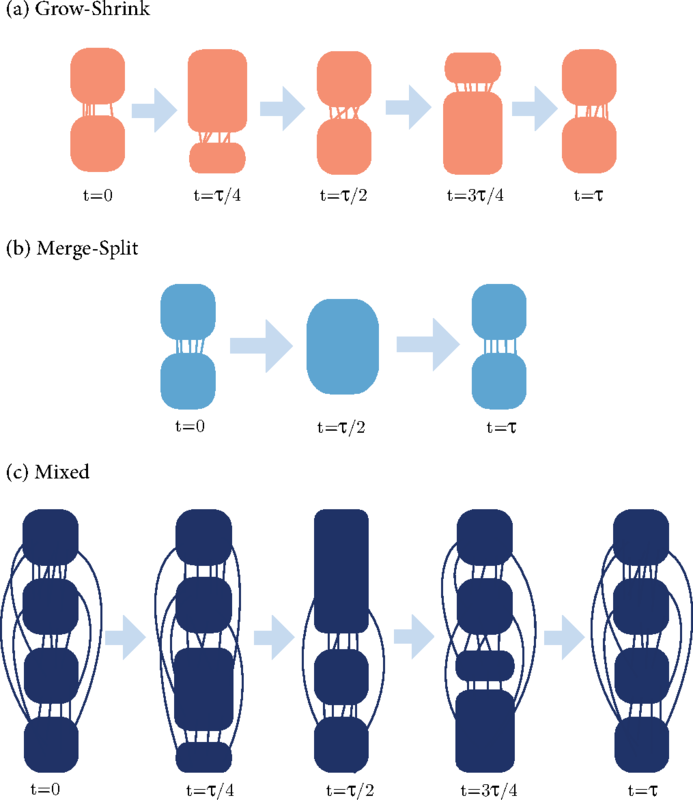
\includegraphics[width=0.4\linewidth]{img/Qualite/Granell.png}
\caption{Représentation schématique d'évolution possible d'une structure communautaire de séries de graphes pouvant être générées par la méthode de Granell \emph{et al.}~\cite{Granell2015a}. Image provenant de~\cite{Granell2015a}.}
\label{fig:qualite_Grannell}
\end{figure}

Ces méthodes génèrent ainsi aisément des structures communautaires mais ne permettent de générer que des séries de graphes.

\subsection{Flots de liens}

Dans les flots de liens, il n'existe pas à notre connaissance de travaux étudiant la génération de flots de liens avec une structure communautaire.
Il existe principalement des méthodes étudiant les distributions de temps inter-contacts~\cite{Malmgren2008,Malmgren2009,Vestergaard2014}.
Il y a dans la littérature un large consensus sur le fait que la distribution des temps inter-contacts est souvent à queue lourde (\emph{heavy-tailed}) dans les jeux de données réels~\cite{Karsai2011,Karsai2012a,Kivela2015}.
D'autre part, les temps inter-contacts ne semblent pas suivre un processus de Markov simple car il y a des corrélations et des effets de mémoire entre les apparitions de liens.

Toutes ces méthodes génèrent des flots de liens mais ne considèrent aucune structure.
Quelques méthodes se distinguent de ces travaux et génèrent une structure même s'il ne s'agit pas forcément de structure communautaire.
C'est le cas des travaux de Starnini \emph{et al.}\cite{Starnini2013} et de Zhang \emph{et al.}~\cite{Zhang2015a}.
Dans ces méthodes, un flot de liens est généré à partir d'un système multi-agents où chaque agent se déplace dans un espace 2D borné.
Un lien existe entre deux agents lorsqu'ils sont à distance de communication.
Dans le modèle de Zhang \emph{et al.}, la direction prise par chaque agent n'est pas aléatoire mais en fonction de l'agent voisin étant le plus attractif.
Il s'agit donc d'un modèle de mobilité préférentielle.
Bien que ces méthodes génèrent des structures, il ne s'agit pas de structures communautaires explicites et elles ne peuvent pas être représentées sur les liens du flot de liens.



Barrat \emph{et al.}~\cite{Barrat2013a} proposent une méthode basée sur l'utilisation de marches aléatoires.
Ils utilisent un graphe statique pondéré et orienté qui représente l'ensemble des interactions qui pourront exister dans le flot de liens.
Ce graphe peut provenir de données réelles ou être généré.
\`A partir de ce graphe, différentes marches aléatoires sont simulées.
Chaque marche est caractérisée par un temps de début, un n\oe{}ud de départ, un nombre de sauts et les temps séparant chaque saut.
Ces caractéristiques peuvent être définies arbitrairement ou selon des distributions apprises sur des jeux de données.
Chaque marche de $k$ sauts donne lieu à une liste d'interactions formant une chaîne: $\{(t_1,u0,u1), ..., (t_k,u_{k-1}, u_k)\}$.
Lors de la marche aléatoire, le prochain lien est choisi en fonction de son poids dans le graphe pondéré et le poids du lien choisi est décrémenté de $1$ dans le graphe pondéré.
Un lien ne peut être choisi que si son poids est supérieur à $0$.
L'union des marches simulées forme ainsi le flot de liens.


Si le graphe statique utilisé possède une structure communautaire, il est possible que le flot de liens généré ait également une structure communautaire.
Cependant cette dépendance ne permet pas de générer des structures communautaires qui soient invisibles dans le graphe statique.
Dans l'exemple \emph{Merge-Split} de la figure~\ref{fig:qualite_Grannell}, il existe deux communautés aux instants $t=0$ et $t=\tau$ mais ces deux communautés sont fusionnées à l'instant $t=\tau/2$.
Il existe donc une structure communautaire dans le réseau dynamique initial mais cette structure n'est pas directement identifiable dans le graphe agrégé.
C'est pourquoi il se peut qu'il n'existe aucune structure communautaire dans le flot de liens généré à partir de ce graphe statique.


\resume{
Dans le cas des séries de graphes, il existe des propositions de générateur avec structure communautaire.
Dans le cadre de flots de liens, les générateurs ne permettent pas ou alors que partiellement de générer une structure communautaire.
}

\section{Méthode de génération}
\label{sec:versqualite_methode}

Nous définissons maintenant notre générateur de flots de liens sans durée ayant une structure communautaire.
Notre approche est similaire au SBM car l'apparition de liens entre deux n\oe{}uds ne dépend que des communautés auxquelles ils appartiennent.
Plus ils ont de communautés en commun, plus il existera de liens entre ces n\oe{}uds.
S'ils n'ont aucune communauté en commun, alors, il n'y aura pas ou peu de liens entre ces n\oe{}uds.
Tout comme le SBM, nous utilisons un graphe d'affiliation des n\oe{}uds aux communautés où il existe un lien entre un n\oe{}ud et une communauté si le n\oe{}ud appartient à la communauté.

Dans le cadre de notre générateur, une communauté représente un intérêt, et une personne peut naturellement avoir plusieurs intérêts.
Ainsi en reprenant l'exemple précédent, il existe dans le graphe d'affiliation autant de n\oe{}uds que de personnes et il existe une communauté représentant les entraînements de sport du mercredi soir, une représentant une réunion de famille, \emph{etc}.

De ce graphe biparti, les approches statiques infèrent la probabilité que deux n\oe{}uds soient reliés par un lien.
Dans le contexte de flots de liens, il ne suffit pas de calculer la probabilité qu'un lien apparaisse dans le cadre d'une communauté.
Il faut générer un ensemble d'interactions temporelles entre ces deux n\oe{}uds au sein de cette communauté.
C'est pourquoi à chaque communauté est associé un processus stochastique de génération de liens dépendant du temps.
Ainsi, chaque communauté partagée par deux n\oe{}uds donne lieu à la génération d'un ensemble de liens selon le processus stochastique de cette communauté.
Par exemple, le processus stochastique de la communauté sport est défini par une forte activité durant les séances d'entraînement et une faible activité en dehors de ces instants.
Une représentation schématique de cette situation est présentée dans la figure~\ref{fig:qualite_Generator}.



\begin{figure}
\centering
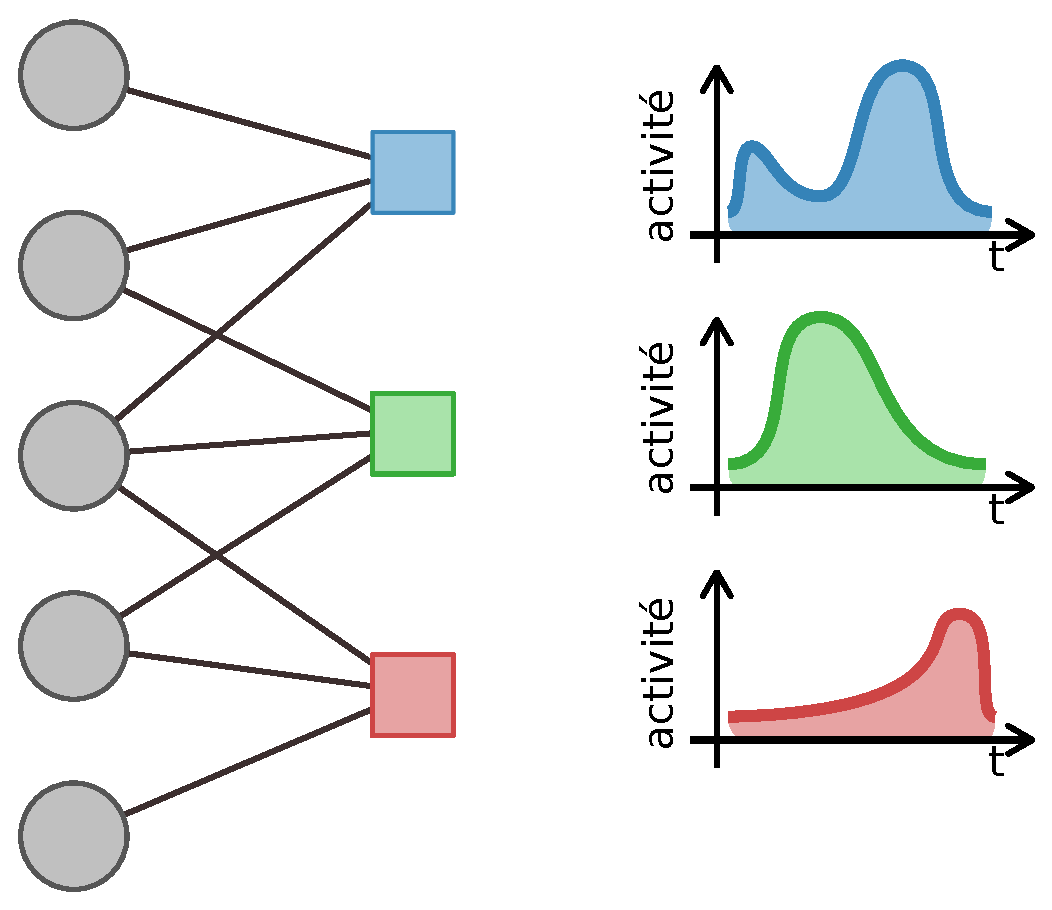
\includegraphics[width=0.45\textwidth]{img/Qualite/Generator}
\caption{Schéma représentant la structure communautaire d'un flot de liens dans notre générateur.
\`A gauche: un n\oe{}ud rond est un individu et un n\oe{}ud carré est une communauté.
\`A droite: Activité au cours du temps associée à chaque communauté du graphe biparti de gauche.}
\label{fig:qualite_Generator}
\end{figure}

Le problème est alors de définir un processus de génération pour chaque communauté.
Un processus de Poisson homogène permet de générer des temps inter-contacts suivant une loi exponentielle de paramètre $\lambda$.
Cela implique que des liens apparaissent toujours avec une moyenne de $\lambda$ liens par unité de temps.
Or, cette hypothèse d'activité constante au cours du temps n'est pas cohérente avec notre modèle.
Par exemple, les réunions de familles sont souvent calmes au début puis deviennent plus animées par la suite.
Il faut donc pouvoir faire varier l'intensité de l'activité au cours du temps.
Si $\lambda$ varie, alors un processus de Poisson non-homogène est simulé.
C'est pourquoi nous considérons des processus de Poisson non-homogènes pour générer des liens au sein d'une communauté.

\bigskip

Avec $N(t)$ représentant le nombre de liens existants dans l'intervalle $[\alpha,t]$, le nombre de liens apparaissant entre deux instants, $a$ et $b$, suit alors la distribution suivante:
\begin{equation}
P [N(b) - N(a) = k] = \frac{e^{-\Lambda_{a,b}} (\Lambda_{a,b})^k}{k!} \qquad k= 0,1,\ldots \ ,
\end{equation}
où $\Lambda_{a,b}=\int_a^b \lambda(t)\,dt$.
Par conséquent la probabilité qu'il y ait un et un seul lien ($k=1$) dans l'intervalle suit une loi exponentielle de paramètre $\Lambda_{a,b}$: $P [N(b) - N(a) = 1]=\Lambda_{a,b}e^{-\Lambda_{a,b}}$.
La fonction de répartition associée est $P [N(b) - N(a) \leq x]= 1 - ^{-\Lambda_{a,b}x}$.
Pour des valeurs de $a$ et $x$ fixées, cette fonction de répartition est une fonction continue, croissante avec $b$ et elle est injective.
Cette fonction est également surjective si elle est strictement croissante, c'est à dire si $\Lambda_{a,b}$ est strictement croissant.

Le processus pour générer un ensemble de liens entre deux n\oe{}uds dans une communauté est le suivant: la génération commence à l'instant $t_0=\alpha$, puis il est nécessaire de générer $t_1$, l'instant d'apparition du prochain lien.
Cet instant est le premier instant $t'$ tel que $N(t')- N(t_0)=1$ et il est relié à la probabilité suivante: $P [N(t_1) - N(t_0) \leq 1] = 1]=1-e^{-\Lambda_{t_0,t_1}}$.
Or, cette application est bijective.
Il est donc possible de retrouver à partir d'une probabilité l'instant lié à cette probabilité.
Il s'agit d'une méthode d'inversion.
Ainsi pour générer $t_1$, on génère une valeur aléatoire uniformément répartie entre $0$ et $1$ puis il suffit de retrouver l'instant lié à cette probabilité.
Comme $\lambda(t)$ peut être quelconque, le calcul de l'instant lié à cette probabilité se fait via une recherche dichotomique.
C'est à dire qu'un instant d'apparition de lien est choisi au hasard puis modifié pour se rapprocher de la probabilité voulue.
Pour générer les apparitions de liens suivantes, il suffit de recommencer ce processus à partir de $t_1$ et de chercher l'instant $t_2$ tel que $N(t_2)- N(t_1)=1$.
Un exemple de génération de temps d'apparition est présenté dans la figure~\ref{fig:qualite_Activation}.


\begin{figure}
\centering
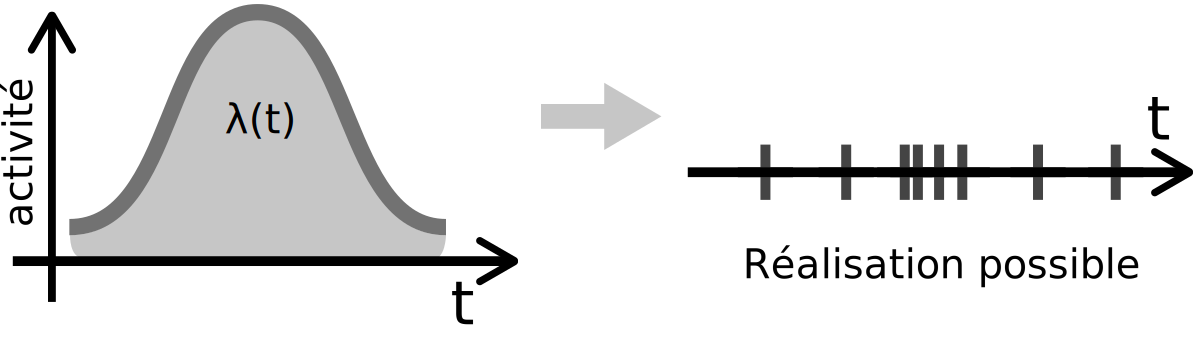
\includegraphics[width=0.6\linewidth]{img/Qualite/Activation}
\caption{Exemple des temps d'activation du lien entre deux n\oe{}uds donnés.}
\label{fig:qualite_Activation}
\end{figure}


En répétant le processus ci-dessus pour chaque paire de n\oe{}uds appartenant à une même communauté, on obtient un flot de liens avec une structure communautaire sur les liens.

\subsection{Caractéristiques du générateur}

Nous discutons maintenant des caractéristiques de ce générateur.
Tout d'abord au sein d'une communauté, il est possible de représenter énormément d'activités temporelles différentes.
Une intensification (resp. baisse) des interactions au cours du temps est représentée par une activité croissante (resp. décroissante).
Il est possible de représenter des réunions cycliques par une activité périodique. 
Ce modèle d'activation des liens reste cependant une approximation car il n'y a aucune prise en compte des possibles corrélations au sein d'une communauté.
De même, les paires de n\oe{}uds d'une communauté correspondent des processus indépendants et identiquement distribués.
Il n'y a donc au sein d'une communauté aucune différence entre les n\oe{}uds.
Il n'est, de plus, pas possible de représenter l'intégration progressive de n\oe{}uds dans une communauté.

Vis-à-vis de l'ensemble des communautés, le modèle est encore une fois assez libre car un n\oe{}ud peut appartenir à plusieurs communautés.
Chaque communauté est traitée de manière indépendante et une même paire de n\oe{}uds peut donner lieu à la génération de liens de différentes communautés.
Ainsi même si les n\oe{}uds sont équivalents au sein d'une communauté, il existe tout de même une hétérogénéité des n\oe{}uds en fonction du nombre de communautés auxquels ils appartiennent.

\bigskip

Avec cette formulation, le générateur dépend du graphe biparti d'affiliation des n\oe{}uds aux communautés et de l'activité temporelle de chaque communauté.
L'approche que nous suivons est purement générative.
Le but n'est donc pas d'inférer ces paramètres sur un exemple mais de pouvoir les fixer manuellement.
Afin de faciliter l'utilisation de ce générateur, nous utilisons différentes méthodes pour fixer ces nombreux paramètres dans la sous-section~\ref{subsec:versqualite_qualite_param}.


\section{Applications}
\label{sec:versqualite_Applications}


%Les paramètres générant le flot de liens peuvent être minutieusement choisis afin que le flot de liens exhibe des caractéristiques spécifiques.
%C'est cette approche que nous utilisons pour tester deux méthodes de détection statique dans la sous-section~\ref{sec:versqualite_statique}.
%
%Les paramètre peuvent être choisi aléatoirement selon certain critère afin de générer des structures plus diverses.
%C'est cette approche que nous utilisons pour l'étude de fonctions de qualité dans la sous-section~\ref{sec:versqualite_qualite}.



\subsection{Étude de méthodes statiques appliquées aux flots de liens}
\label{sec:versqualite_statique}

Lors de la génération de graphes statiques avec structure communautaire chevauchante, il y a principalement deux critères influençant une réalisation: le chevauchement de la structure et le rapport entre densité intérieure et extérieure à une communauté.
Dans le cas des flots de liens, il faut aussi ajouter le chevauchement temporel.
Afin de faciliter l'étude, nous ne générons aucun lien en dehors des communautés définies.
C'est pourquoi les différentes situations dépendent uniquement du recouvrement topologique et temporel des communautés.
 
Les flots de liens que nous générons contiennent $15$ n\oe{}uds pendant $30$ unités de temps et il y existe cinq communautés ayant chacune une durée de $10$ unités de temps.
Afin de simplifier la méthode de test, chaque communauté a une activité constante de $0.5$ durant l'intervalle où elle existe.
Avec ces paramètres fixés, nous faisons varier le chevauchement topologique de trois manières différentes qui sont représentées dans les figures suivantes:

\begin{description}
\item[\ref{fig:versqualite_gen_test1}] chaque communauté est bien séparée des quatre autres. Il s'agit de l'exemple le plus simple car il n'y a aucun chevauchement topologique des communautés;
\item[\ref{fig:versqualite_gen_test2}] il existe un chevauchement topologique entre la communauté $3$ et les autres;
\item[\ref{fig:versqualite_gen_test3}] il y a, en plus du chevauchement avec la communauté $3$, un faible chevauchement topologique entre les communautés $1$ et $2$ et entre les communautés $4$ et $5$.
\end{description}


 
\begin{figure}
\centering
	\begin{subfigure}{0.3\textwidth}
		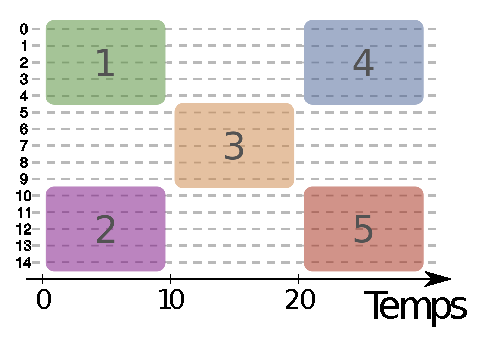
\includegraphics[width=\textwidth]{img/Qualite/topologie1.eps}
		\caption{}
		\label{fig:versqualite_gen_test1}
	\end{subfigure}
	\begin{subfigure}{0.3\textwidth}
		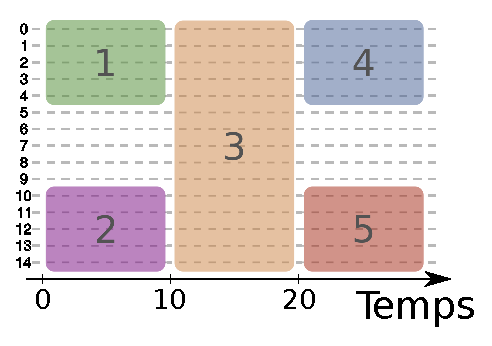
\includegraphics[width=\textwidth]{img/Qualite/topologie2.eps}
		\caption{}
		\label{fig:versqualite_gen_test2}
	\end{subfigure}
	\begin{subfigure}{0.3\textwidth}
		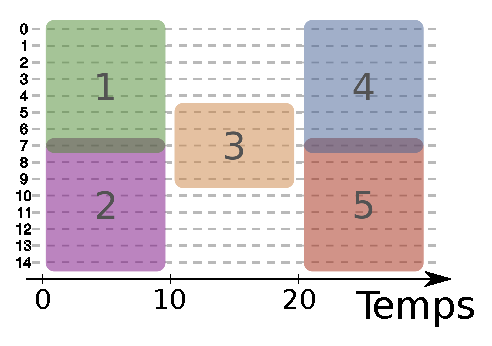
\includegraphics[width=\textwidth]{img/Qualite/topologie3.eps}
		\caption{}
		\label{fig:versqualite_gen_test3}
	\end{subfigure}
%	\begin{subfigure}{0.3\textwidth}
%		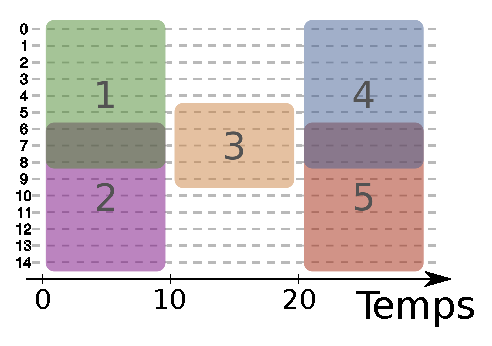
\includegraphics[width=\textwidth]{img/Qualite/topologie4.eps}
%		\caption{}
%		\label{fig:versqualite_gen_test4}
%	\end{subfigure}	
	\caption{Représentation schématique de trois types de flot de liens ayant une structure communautaire avec cinq communautés.
	Chaque rectangle de couleur représente une communauté ayant une activité constante.}
	\label{fig:versqualite_gen_test}
\end{figure}

\bigskip
Pour ces trois types de flots de liens, nous avons appliqué Louvain, une méthode d'optimisation de modularité~\cite{Blondel2008a} et CarOp, une méthode \emph{ego}-centrée~\cite{Danisch2012} sur une projection du flot de liens en un graphe statique.
La méthode CarOp permet de trouver une communauté \emph{ego}-centrée à partir d'un n\oe{}ud du graphe.
Il est donc nécessaire de fournir un lien initial qui servira à retrouver les communautés générées.
Nous choisissons pour chaque communauté générée un lien apparaissant au milieu de sa duré de vie; par exemple un lien à l'instant $15$ est choisi pour initialiser une communauté qui sera \emph{a priori} proche de la communauté $3$.


Nous avons défini précédemment une projection du flot de liens en un graphe statique mais uniquement dans le cas où les liens ont une durée.
Dans les flots de liens générés ici, il n'y a pas de durée sur les liens.
C'est pourquoi nous utilisons une projection différente qui transforme le flot de liens en un graphe statique pondéré.
Chaque lien du flot est toujours représenté par un n\oe{}ud dans le graphe statique et il y a un lien entre deux n\oe{}uds du graphe si les liens correspondants ont un n\oe{}ud en commun.
Afin de tenir compte de la séparation temporelle, un lien dans le graphe statique est pondéré par une fonction décroissante du temps séparant les deux liens dans le flot.
Nous avons choisi comme fonction décroissante: $e^{-\lambda d}$ où $d$ est le temps séparant les deux liens et $\lambda$ une constante positive.
Ainsi, les poids dans la projection sont répartis entre $0$ et $1$.
Plus $\lambda$ a une valeur importante, plus le poids d'un lien est faible.
Par exemple pour $\lambda=3$, une séparation temporelle de $1$ unité de temps donne lieu à poids de $0.05$ dans la projection.
Dans cette situation, le graphe de la projection ne capture plus vraiment de relations topologiques car un lien n'est alors relié avec un poids non négligeable qu'avec ses voisins les plus proches.
Dans le cas inverse, quand $\lambda$ est égal à zéro, la projection du flot de liens est complètement identique au \emph{line-graph} du multigraphe agrégé.
Dans la suite, nous avons à chaque fois fait varier $\lambda$ de manière exhaustive.

Lors de nos tests, nous nous sommes appuyés sur notre outil de visualisation pour comparer visuellement\,\footnote{Une évaluation plus quantitative avec la \emph{NMI} est possible mais ne semble pas nécessaire car les différences entre les partitions sont clairement visibles dans la visualisation.} la vérité de terrain, les partitions trouvées par Louvain et CarOp selon le $\lambda$ choisi.

\bigskip

Dans la situation la plus simple représentée dans la figure~\ref{fig:versqualite_gen_test1}, nous observons que les deux méthodes sont capables de retrouver la vérité de terrain.

Dans la situation représentée dans la figure~\ref{fig:versqualite_gen_test2}, la vérité de terrain est retrouvée par CarOp mais non par Louvain.
Dans les partitions trouvées par Louvain, la communauté $3$ n'est jamais détectée, peu importe la valeur de $\lambda$ utilisée pour la projection.
Selon la valeur de $\lambda$, les liens de la communauté $3$ sont soit distribués entre les autres communautés, soit répartis en plusieurs communautés autonomes.
Comme cette méthode optimise la modularité sur une structure proche du \emph{line-graph} d'un multigraphe, elle est similaire aux méthodes proposées par Evans et Lambiotte~\cite{Evans2009} que nous avons présentées dans la section~\ref{sec:expected_travaux}.
Elle souffre donc des mêmes biais\,\footnote{Plus une clique d'un graphe est grande, moins sa transformation dans le \emph{line-graph} est dense.}.

Dans la situation représentée dans la figure~\ref{fig:versqualite_gen_test3}, la vérité de terrain est retrouvée par Louvain mais non par CarOp.
Comme les communautés sont petites, la méthode de Louvain arrive à détecter les différentes communautés.
La méthode CarOp, quant à elle, n'est pas capable de différencier les communautés $1$ et $2$.
Ces deux communautés sont fusionnées en une seule par CarOp.
En effet, CarOp utilise la proximité des liens dans la projection.
Or, un lien au début de la communauté $1$ est plus proche des liens au débuts de la communauté $2$ que des liens à la fin de la communauté $1$.
C'est pourquoi CarOp ne différencie pas les communautés $1$ et $2$.

%Dans la situation représentée dans la figure~\ref{fig:versqualite_gen_test4}, la vérité de terrain n'est retrouvée ni par Louvain ni par CarOp.
%Comme la situation dans la figure~\ref{fig:versqualite_gen_test4} est proche de celle de la figure~\ref{fig:versqualite_gen_test3}, il est normal que CarOp ne parvienne toujours pas à différencier les communautés $1$ et $2$.
%Pour la méthode de Louvain, les communautés $1$ et $2$ ne sont également pas détectées.
%Pour des valeurs faibles de $\lambda$, les communautés $1$ et $2$ sont séparées en $4$ ou $5$ communautés sans logique apparente.
%Pour des valeurs élevées de $\lambda$, il existe bien deux communautés correspondant aux communautés $1$ et $2$ mais la partie chevauchante est complètement intégrée dans l'une de ces deux communautés.



\resume{
Il s'agit de premiers tests sur des méthodes existantes de détection de communautés sur des projections du flot de liens en graphes pondérés.
Les méthodes que nous avons testées ne permettent pas de détecter la vérité de terrain dans l'ensemble des situations générées.
Ce fait est attendu car nous les appliquons sur des projections du flot de liens.
Il est toutefois intéressant de noter qu'il est possible de retrouver la vérité de terrain par une méthode statique sous certaines conditions qui restent encore à pleinement comprendre.
}

\subsection{Vers des fonctions de qualité dans les flots de liens}
\label{sec:versqualite_qualite}

Les approches statiques ne permettent pas toujours de détecter la vérité de terrain.
Nous faisons donc une première proposition de fonction de qualité évaluant les partitions de liens des flots de liens et nous nous appuyons sur notre générateur et sur des partitions trouvées empiriquement pour étudier les caractéristiques de cette fonction de qualité.





\subsubsection{Jeux de paramètres pour la génération de flots de liens}
\label{subsec:versqualite_qualite_param}
Le générateur dépend de beaucoup de paramètres qui sont difficiles et fastidieux à choisir manuellement pour de grands exemples.
Il faut définir un graphe biparti d'affiliation des individus aux communautés et l'activité temporelle de chaque communauté.
Afin de simplifier ce processus, il est possible de s'appuyer sur un générateur de graphe biparti.

De manière analogue au graphe, un graphe biparti peut être généré de telle sorte qu'il ait une densité donnée ou qu'il ait une distribution des degrés particulière.
Nous faisons le choix de générer des graphes bipartis où le degré moyen des n\oe{}uds est fixé et où chaque individu est relié à au moins une communauté.
Ainsi, un degré moyen de $1$ implique qu'il n'y a aucun chevauchement entre les communautés.
Un degré moyen de $1.8$ implique qu'un n\oe{}ud d'une communauté est relié en moyenne à $0.8$ autres communautés et donc qu'une communauté de taille $k$ partage des n\oe{}uds avec au maximum $0.8k$ autres communautés.

Pour l'activité des communautés, nous imposons la même activité constante et la même durée d'activité pour toutes les communautés.
Il suffit de décider du moment où l'intervalle débute pour définir l'activité d'une communauté.
Pour une durée fixe $\Delta$, nous choisissons de tirer de manière uniforme le temps de début d'une communauté dans $[\alpha,\omega-\Delta]$.
Ainsi, plus le flot de liens est long par rapport à la durée d'activité des communautés, moins il y aura de chevauchement temporel.

\bigskip
Pour générer un flot de liens, le nombre de paramètres est maintenant plus restreint.
Il suffit de fixer manuellement le nombre de n\oe{}uds, le nombre de communautés, le degré moyen dans le graphe biparti, la durée d'une communauté, l'activité d'une communauté et la durée totale du flot de liens.
Les trois premiers paramètres permettent de contrôler le chevauchement topologique alors que les trois derniers permettent de contrôler le chevauchement temporel.

\subsubsection{Proposition de fonctions de qualité}

Nous l'avons évoquée à de nombreuses reprises.
La modularité est une fonction de qualité évaluant une partition de n\oe{}uds, $\mathcal{V}=\{V_1,..,V_k\}$, d'un graphe.
Une des formulations pour la calculer est la suivante:
\begin{equation}
Q_G(\mathcal{V}) =  \sum_{i=1}^{k} Q_G(V_i) =\sum_{i=1}^{k} \left( \dfrac{d_{in}(V_i)}{2m}- \left(\dfrac{d(V_i)}{2m}\right)^2\right)\,.
\end{equation}
Pour rappel, $d(V_i)$ est la somme des degrés des n\oe{}uds de $V_i$ et $d_{in}(V_i)$ est la somme des degrés des n\oe{}uds de $V_i$ lorsqu'uniquement les liens inclus dans $V_i \times V_i$ sont considérés.
Il est possible de généraliser la modularité aux flots de liens en considérant une partition des n\oe{}uds à chaque instant.
Cette partition temporelle, $\mathcal{V}(t)$, doit respecter les contraintes d'une partition pour tout instant $t \in [\alpha,\omega]$.
Avec ces notations, on peut calculer la modularité moyenne de $\mathcal{V}(t)$ sur un flot de liens $L$:

\begin{equation}
Q_L(\mathcal{V}) = \dfrac{1}{\omega-\alpha} \int_{\alpha}^{\omega} Q_{G(L_t)}(\mathcal{V}(t)) dt\,.
\label{eq:temp_modu}
\end{equation}

Cette formulation met en avant l'intégrale de la modularité du graphe mais la modularité elle même est une somme sur les groupes de n\oe{}uds.
Nous transformons donc l'équation précédente pour mettre en avant la modularité d'un groupe de n\oe{}uds sur un intervalle de temps.
Si dans la partition temporelle un groupe de n\oe{}ud $V'$ est une communauté sur un intervalle $[\beta, \psi]$ alors sa qualité, $Q_L(V', \beta, \psi)$, peut se calculer de la manière suivante:

\begin{equation}
Q_L(V', \beta, \psi)  = \int_{\beta}^{\psi} \! \dfrac{d_{in}(t,V')}{d(t,V)} - \left( \dfrac{d(V',t)}{d(V,t)} \right)^2  \, dt\, ,
\end{equation}

$d(t,V')$ et $d_{in}(t,V')$ sont définis dans la section~\ref{sec:def_densite} et sont respectivement la somme des degrés temporels des n\oe{}uds de $V_i$ et la somme des degrés temporels des n\oe{}uds de $V_i$ lorsqu'uniquement les liens inclus dans $V_i \times V_i$ sont considérés.
Avec cette formulation, on voit apparaître le degré temporel dans le calcul de cette version de la modularité d'un groupe.
La vérité de terrain générée n'est cependant pas une partition temporelle des n\oe{}uds mais une partition de liens du flot de liens.
Il faut donc adapter la formulation précédente pour manipuler des groupes de liens au lieu de groupes de n\oe{}uds sur un intervalle de temps.
Ainsi, nous définissons la modularité d'un groupe de liens $C_i$:
\begin{equation}
Q_L(C_i)  = \int_{\beta(C_i)}^{\psi(C_i)} \! \dfrac{d(t,C_i)}{d(t,V)} -  \left( \dfrac{d(t,V(C_i))}{d(t,V)} \right)^2 \, dt \,.
\label{}
\end{equation}
Il s'agit de l'intégrale de la différence entre la probabilité qu'un lien appartienne à $C_i$ et la probabilité qu'il existe un lien entre les n\oe{}uds induits par $C_i$.
On définit enfin la qualité d'une partition de liens $\mathcal{C}$:
\begin{equation}
Q_L(\mathcal{C}) = \dfrac{1}{\omega-\alpha} \sum_{C_i \in C} Q_L(C_i)\, .
\label{eq:temp_modu_liens}
\end{equation}

Cependant en considérant un groupe de liens au lieu d'un groupe de n\oe{}uds, la modularité n'est plus bornée entre $-1$ et $1$.
La modularité classique est bornée entre $-1$ et $1$ et par conséquent la version temporelle de la modularité de l'équation~\ref{eq:temp_modu} est également bornée car il s'agit de la moyenne de la modularité au cours du temps.
La modularité temporelle de groupes de liens de l'équation~\ref{eq:temp_modu_liens} n'est pas bornée.
En effet, cette formulation utilise le degré temporel des n\oe{}uds induits ce qui implique qu'un n\oe{}ud peut être considéré à plusieurs reprises par différent groupes de liens.
C'est le cas lorsqu'un n\oe{}ud a des liens appartenant à plusieurs groupes différents.

 

Même si cette version n'est pas bornée, elle permet tout de même d'évaluer une partition de liens en comparant la proportions de liens appartenant au groupe à la proportion attendue dans le modèle de configuration à chaque instant.
De plus, la partition contenant l'ensemble des liens obtient également une qualité nulle.
Elle semble donc être une bonne candidate pour évaluer une partition de liens.

\subsubsection{Résultats}

Avec le générateur d'une part et la modularité temporelle d'autre part, nous avons procédé de manière analogue à ce que nous avons fait pour \emph{Expected Nodes} dans la section~\ref{sec:expected_comp}.
Nous générons plusieurs types de flots de liens en contrôlant le chevauchement temporel et topologique.
Pour chaque flot de liens généré, nous comparons la qualité de trois partitions de liens: \emph{i)} la vérité de terrain ($V$), \emph{ii)} la partition trouvée par la méthode de Louvain sur la projection pondérée du flot de liens ($Lo$)\,\footnote{Nous l'avons définie dans la section~\ref{sec:versqualite_statique}.} et \emph{iii)} la partition triviale où chaque lien est dans sa propre communauté ($S$).
La partition $Lo$ est obtenue de la même manière que dans la section~\ref{sec:versqualite_statique}, c'est-à-dire en gardant la meilleure partition parmi celles trouvées via différentes valeurs de $\lambda$ choisies pour la projection.
Nous n'utilisons pas CarOp car elle ne redonne pas directement une partition de liens mais une couverture de liens.

Les liens du flot de liens généré n'ont pas de durée.
Or, pour utiliser le degré temporel, il est nécessaire que les liens aient une durée.
Nous ajoutons donc une durée $\Delta$ à chaque lien ($\xi(L,\Delta)$) et il est alors nécessaire de simplifier le flot de liens résultant ($\sigma(\xi(L,\Delta))$), afin de pouvoir utiliser la notion de degré temporel.
La simplification d'un flot de liens revient à remplacer deux liens $(b,e,u,v)$ et $(b',e',u,v)$ se chevauchant temporellement par un lien $(min(b,b'),max(e,e'),u,v)$.
Cela ne pose pas de problème lorsque ces liens appartiennent à la même communauté.
C'est délicat lorsqu'ils n'appartiennent pas à la même communauté.
Cette situation est illustrée dans la figure~\ref{fig:qualite_simplification}.

\begin{figure}
\centering
%\subfloat[Inverse cumulative distribution of inter-threads density.]{
	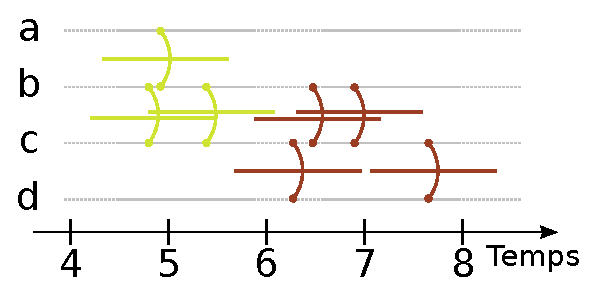
\includegraphics[width=0.65\linewidth]{img/Qualite/inter_flot.eps}
%}
\caption{Flot de liens avec deux communautés en \textcolor{olivegreen}{\textbf{vert}} et \textcolor{briquered}{\textbf{rouge}} où chaque lien a une durée égale à $1.5$.
La simplification de ce flot de liens est problématique pour les liens entre $b$ et $c$ à l'instant $6$.}
\label{fig:qualite_simplification}
\end{figure}

Il est donc nécessaire de différencier la simplification lorsque l'on s'intéresse au degré d'une communauté en particulier ou au degré du flot de liens en général.
Dans le premier cas, on étudie $\sigma(\xi(L(C_i),\Delta))$, le sous-flot induit par les liens de la communauté et dans le second on étudie $\sigma(\xi(L,\Delta))$.
Ces changements, bien que lourds, sont nécessaires pour rendre simple le flot de liens et pouvoir calculer le degré temporel d'une communauté, d'un ensemble de n\oe{}uds et du flot de liens.
Afin de tester plusieurs $\Delta$ rapidement, nous nous sommes appuyés sur l'outil \emph{parallel}~\cite{Tange2011a}.


\bigskip
Pour la génération, nous considérons $100$ n\oe{}uds et $10$ communautés durant chacune $20$ unité de temps avec une activité constante de $0.1$.
Avec une activité de $0.1$, il y a en moyenne deux liens appartenant à la communauté pour chaque paire de n\oe{}uds.
Nous choisissons une durée totale du flot de liens de $50$ ou $200$ pour contrôler le chevauchement temporel.
Nous choisissons un degré moyen dans le biparti de $1.1$ ou $2$ pour contrôler le chevauchement topologique.
Les flots de liens ainsi générés ont entre $1\ 200$ et $4\ 000$ liens selon le chevauchement choisi.

Les valeurs de qualité pour chaque situation et chaque partition en fonction de la durée des liens sont présentées dans la figure~\ref{fig:versqualite_fonc_test}.
On remarque également que la vérité de terrain est la meilleure partition, peu importe le cas de figure lorsque $\Delta$ est supérieur à 2.
Lorsqu'il y a un important chevauchement topologique, figure~\ref{fig:versqualite_fonc_test3} et \ref{fig:versqualite_fonc_test4}, la vérité de terrain a toutefois une qualité plus faible selon la fonction de qualité.
C'est en particulier visible dans la figure~\ref{fig:versqualite_fonc_test3} où le chevauchement temporel est également important.
Dans cette situation, la qualité obtenue par la vérité de terrain est négative alors que la partition contenant l'ensemble des liens a une qualité nulle.
Avoir une qualité négative dans ce cas de figure n'est toute fois pas complètement surprenant car la structure est difficilement discernable avec des chevauchements si importants.

Lorsque $\Delta$ tend vers $0$, la qualité des partitions tend également vers $0$ car le degré moyen tend vers $0$.
Par ailleurs, nous avons remarqué dans la section~\ref{sec:versqualite_statique} que la méthode de Louvain est parfois à même de retrouver la vérité de terrain, notamment lorsque le chevauchement est faible.
Il y a très peu de chevauchement dans la situation représentée dans la figure~\ref{fig:versqualite_fonc_test2} et nous observons que la partition $Lo$ est identique à la vérité de terrain pour ce cas particulier.
Enfin, la partition où chaque lien est dans sa propre communauté obtient toujours une qualité élevée lorsque $\Delta$ est compris entre $10^{-2}$ et $2$.


\begin{figure}[h]
\centering
	\begin{subfigure}{0.495\textwidth}
		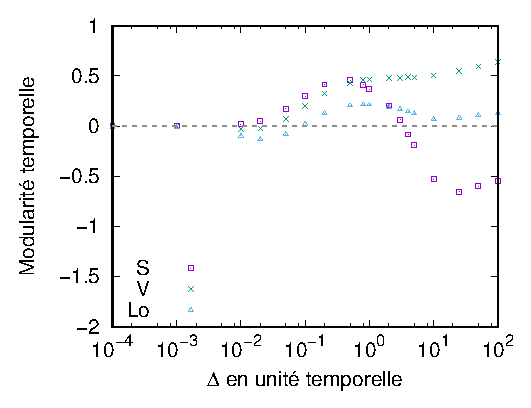
\includegraphics[width=\textwidth]{img/Qualite/Fonc/comp_1_T_50_O_1_1_Q_1.eps}
		\caption{$O=1.1$ \& $T=50$}
		\label{fig:versqualite_fonc_test1}
	\end{subfigure}
	\begin{subfigure}{0.495\textwidth}
		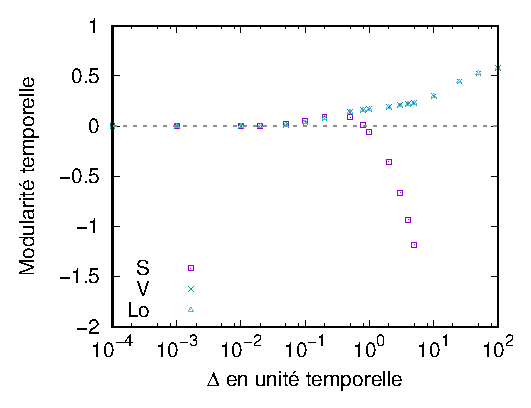
\includegraphics[width=\textwidth]{img/Qualite/Fonc/comp_0_1_T_200_O_1_1_Q_1.eps}
		\caption{$O=1.1$ \& $T=200$}
		\label{fig:versqualite_fonc_test2}
	\end{subfigure}
	
	\vspace*{0.7cm}
	\begin{subfigure}{0.495\textwidth}
		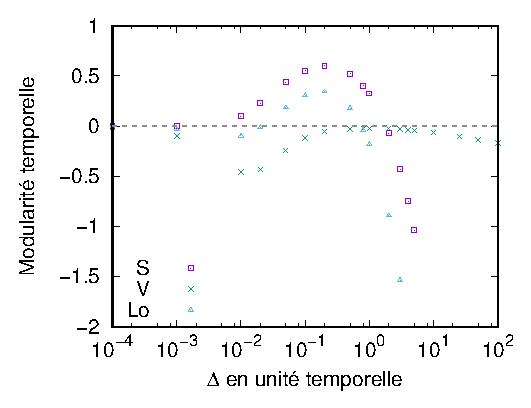
\includegraphics[width=\textwidth]{img/Qualite/Fonc/comp_50_T_50_O_2_Q_1.eps}
		\caption{$O=2$ \& $T=50$}
		\label{fig:versqualite_fonc_test3}
	\end{subfigure}
	\begin{subfigure}{0.495\textwidth}
		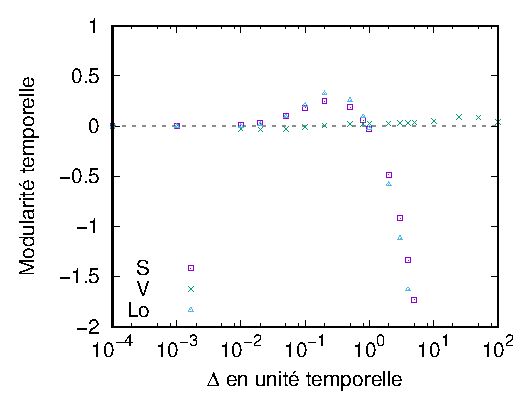
\includegraphics[width=\textwidth]{img/Qualite/Fonc/comp_100_T_200_O_2_Q_1.eps}
		\caption{$O=2$ \& $T=200$}
		\label{fig:versqualite_fonc_test4}
	\end{subfigure}	
	\caption{Évaluation, en fonction de la durée $\Delta$ ajoutée à chaque lien, \emph{i)} de la partition vérité de terrain ($V$), \emph{ii)} de la partition trouvée par la méthode de Louvain ($Lo$) et \emph{iii)} de la partition où chaque lien est dans sa propre communauté $(S)$.
	Les quatre schémas correspondent à différents choix de chevauchement topologique $(O)$ et temporel ($T$).}
	\label{fig:versqualite_fonc_test}
\end{figure}
\bigskip

Ces observations permettent de tirer des premières conclusions sur cette fonction de qualité.
Tout d'abord, la durée des liens a un impact fort sur l'évaluation d'une partition.
Par exemple lorsque la durée est courte, notre fonction de qualité n'évalue pas la vérité de terrain comme la meilleure partition.
Ce phénomène pourrait être dû au fait qu'il n'existe que très peu de liens présents simultanément lorsque $\Delta$ est faible.

Le chevauchement topologique semble également avoir un impact plus important sur les évaluations que le chevauchement temporel.
Cet impact n'est en revanche pas le même pour toutes les partitions.
Pour la vérité de terrain, le chevauchement topologique diminue la qualité alors que pour la partition où chaque est lien est dans sa propre communauté, le chevauchement temporel augmente la qualité.

\resume{
La transposition de la modularité permet d'évaluer des partitions de liens d'un flot de liens.
Cette fonction de qualité réussit à évaluer la vérité de terrain comme la meilleure fonction de qualité dans certaines conditions, lorsque les liens durent suffisamment longtemps.
Cependant, ces travaux ne sont que préliminaires et il est nécessaire d'étudier d'autres cas de figure avant de comprendre cette fonction de qualité.
Il est en particulier important de tester d'autres partitions trouvées empiriquement, notamment avec un algorithme d'optimisation dédié.
}

\section{Conclusion}

Dans ce chapitre, nous nous sommes intéressés à la génération de flots de liens avec une structure communautaire sur les liens.
Il s'agit de la première méthode de ce genre car les méthodes existantes se focalisent sur la génération de flot de liens ayant des distributions des temps inter-contact similaires à celles observées dans les jeux de données réels.

\bigskip

Notre approche est différente.
Nous modélisons l'existence de groupes de n\oe{}uds communiquant pendant des intervalles de temps donnés.
Ainsi, il est possible de simuler des événements durant lesquels des liens apparaissent entre les personnes concernées par ces événements.
Pour ce faire, notre méthode s'inspire du SBM.
Il faut définir \emph{i)} un graphe biparti d'affiliation des n\oe{}uds aux communautés et \emph{ii)} l'activité temporelle de chaque communauté.
Une fois ces paramètres définis, des liens entre deux n\oe{}uds sont générés en fonction de processus de Poisson non-homogènes qui sont spécifiques aux communautés partagées par ces deux n\oe{}uds.

\bigskip

Grâce à ce générateur, nous avons pu tester deux méthodes de détection de communautés sur des projections du flot de liens en graphes statiques pondérés.
Ces premiers résultats sont très intéressants car ces méthodes sont parfois à même de retrouver la vérité de terrain alors qu'elles se basent sur un graphe statique.
Cependant lorsque le chevauchement topologique est important, les méthodes statiques que nous avons testées n'ont pas retrouvé la vérité de terrain.
Il est donc nécessaire de proposer des méthodes pour évaluer et identifier des partitions de liens dans les flots de liens.

\bigskip

Nous avons donc proposé une première fonction de qualité proche de la modularité.
Nous l'avons testée sur des flots de liens présentant différents chevauchement topologiques et temporels.
Sur chaque flot de liens, nous avons évalué la vérité de terrain, une partition trouvée empiriquement et une partition triviale.
Les résultats sont encourageants car la vérité de terrain est souvent évaluée comme la meilleure partition.
Cependant, il est nécessaire d'étudier d'autres cas de figure avant de comprendre cette fonction de qualité.
En particulier, il est important de tester d'autres partitions afin de s'assurer que la qualité de la vérité de terrain soit proche de l'optimum.


\subsection{Perspectives}
Ces premiers travaux concernent un domaine qui n'a, à notre connaissance, jamais été étudié auparavant.
Il y a donc de nombreuses possibilités pour l'amélioration de ce générateur.


Pour qu'un générateur soit utile, il doit générer des structures vraisemblables.
Il est par exemple peu judicieux d'utiliser un graphe généré selon le modèle de Erdös-Rényi pour représenter un réseau social.
C'est une question que nous n'avons pas abordée jusqu'à maintenant mais qui est primordiale.
Le modèle de génération que nous utilisons est très général.
C'est le choix des paramètres qui rend les flots de liens générés vraisemblables ou non.
Il faut donc étudier comment fixer ses paramètres.

Il est par exemple possible de changer l'activité des communautés pour que leur densité et leur durée soient similaires à celles observées dans un jeu de données.
De même, il serait intéressant d'évaluer quel serait un graphe d'affiliation vraisemblable dans le cas des flots de liens.
Pour ce faire, les données de courriels du chapitre~\ref{chap:mailing} et les groupes pertinents détectés dans le chapitre~\ref{groupesDense} peuvent être d'une grande utilité.

En plus de ces premiers aspects, il est également possible de modifier le modèle de génération pour le rendre plus flexible au prix de l'ajout d'autres paramètres.
Par exemple, les liens générés n'ont pas de durée.
Il serait utile de tirer la durée d'un lien selon une distribution donnée.
Se pose alors la question de la cohérence entre la durée d'un lien et le processus de Poisson non-homogène sous-jacent: est-il normal de générer un lien de longue durée durant une activité faible de la communauté?
Pour répondre à ce genre de question, il est nécessaire de s'appuyer sur des observations empiriques.

Enfin, une des hypothèses de notre générateur est l'équivalence des n\oe{}uds au sein d'une communauté.
Il se peut en effet que certains n\oe{}uds soient plus actifs que d'autres.
Un moyen de prendre en compte cette diversité est d'incorporer un système d'attachement préférentiel.
Dans les graphes, l'attachement préférentiel se définit de la manière suivante: chaque n\oe{}ud a un score de "popularité"~\footnote{Le degré est généralement utilisé comme score de popularité.} qui détermine la propension des autres n\oe{}uds à créer un lien avec lui.
Ainsi plus un n\oe{}ud est populaire, plus il acquiert de liens avec les autres n\oe{}uds.
Dans le cadre de la génération de flots de liens, il serait possible que le processus de génération des liens entre deux n\oe{}uds ne dépende plus uniquement de la communauté mais également de la popularité respective des n\oe{}uds.
Cette "popularité", temporelle ou non, devrait également être fixée par l'utilisateur mais elle permettrait de mettre en avant un n\oe{}ud dominant au sein d'une communauté.





